\newcommand{\uch}{{\color{black}\bullet}} % unchanged element
\newcommand{\ch}{{\color{red}*}}
\begin{frame}
  \frametitle{Householder transform}
  
  \begin{columns}[T]
    
    \column{0.5\textwidth}
    
    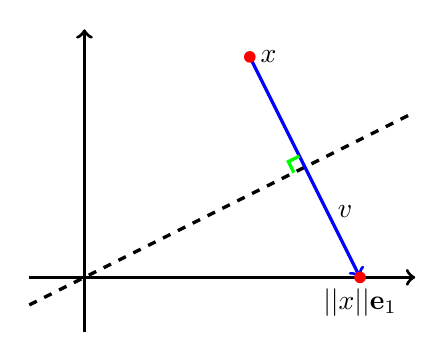
\begin{tikzpicture}[scale=0.7]
      \draw[very thick, ->] (-1,0) -- (6,0);
      \draw[very thick, ->] (0,-1) -- (0,4.5);
      \draw[very thick, dashed] (-1,-0.5) -- (6,3);
      \draw[blue, very thick, ->] (3, 4) coordinate (c1) 
      -- (5,0) coordinate (c2)
      node[black, pos=0, right]{$x$}
      node[black, pos = 0.7, right]{$v$} 
      node[black, pos = 1, below] {$||x|| \mathbf{e}_1$};
      \fill[red] (c1) circle (3pt);
      \fill[red] (c2) circle (3pt);
      % draw the perpendicular symbol.
      % coordinates are 
      % (4-2s, 2-s) -> (4-3t, 2+s) -> (4-t, 2+2t)
      \draw[very thick, green] 
      (4-2*0.1, 2-0.1) --
      (4-3*0.1, 2+0.1) --
      (4-0.1, 2+2*0.1);
    \end{tikzpicture}
    
    \column{0.5\textwidth}
    
    \[
    x=
    \begin{pmatrix}
      x_1 \\
      x_2 \\
      \vdots \\
      x_n \\
    \end{pmatrix}
    \overset{\text{rotation}}{\to}
    \begin{pmatrix}
      ||x|| \\
      0 \\
      \vdots \\
      0 \\
    \end{pmatrix}    
    \]
    
    \[
    v=||x||e_1 - x
    \] gives {\color{cyan} Householder reflection}:
    \[
    H= \mathbf{I} - 2\frac{vv^\top}{v^\top v}
    \]
    Properties of $H$:
    \[
    H^\top=H; \quad H^\top H = \mathbf{I}
    \]
    
  \end{columns}

\end{frame}

\begin{frame}
  \frametitle{Givens rotation}
  For a given matrix $A$, just rotate the ith and (i+1)th 
  row such that the subdiagonal element $A_{i+1,i}=0$.
  \[
  G(i) = 
  \begin{bmatrix}
    1 & & & & \\
    & 1 & & & \\
    & & \vdots & \vdots & \\
    & \cdots & \cos(\theta) & -\sin(\theta) & \cdots \\
    & \cdots & \sin(\theta) & \cos(\theta) & \cdots \\
    & & \vdots & \vdots & \\
    & & & & 1 
  \end{bmatrix}
  \,,
  \]
  where $\tan(\theta)=A_{i,i}/A_{i+1,i}$. 
\end{frame}

\begin{frame}
  \frametitle{Hessenberg-triangular form}
  {\color{green}Example:} three $[5\times 5]$ matrices.
  \[
  \begin{matrix}
    J_3 & J_2 & J_1 \\
    \begin{bmatrix}
      \uch & \uch & \uch & \uch & \uch \\
      \uch & \uch & \uch & \uch & \uch \\
      \uch & \uch & \uch & \uch & \uch \\
      \uch & \uch & \uch & \uch & \uch \\
      \uch & \uch & \uch & \uch & \uch \\
    \end{bmatrix}
    &
    \begin{bmatrix}
      \uch & \uch & \uch & \uch & \uch \\
      \uch & \uch & \uch & \uch & \uch \\
      \uch & \uch & \uch & \uch & \uch \\
      \uch & \uch & \uch & \uch & \uch \\
      \uch & \uch & \uch & \uch & \uch \\
    \end{bmatrix}
    &
    \begin{bmatrix}
      \uch & \uch & \uch & \uch & \uch \\
      \uch & \uch & \uch & \uch & \uch \\
      \uch & \uch & \uch & \uch & \uch \\
      \uch & \uch & \uch & \uch & \uch \\
      \uch & \uch & \uch & \uch & \uch \\
    \end{bmatrix}
  \end{matrix}
  \]
  {\color{green} Step 1} :
  insert an appropriate $\mathbf{I}=H^\top H$ between $J_2$ and $J_1$ :
  \[
  \begin{matrix}
    J_3 & {\color{red} J'_2} & {\color{red} J'_1} \\
    \begin{bmatrix}
      \uch & \uch & \uch & \uch & \uch \\
      \uch & \uch & \uch & \uch & \uch \\
      \uch & \uch & \uch & \uch & \uch \\
      \uch & \uch & \uch & \uch & \uch \\
      \uch & \uch & \uch & \uch & \uch \\
    \end{bmatrix}
    &
    \begin{bmatrix}
      \ch & \ch & \ch & \ch & \ch \\
      \ch & \ch & \ch & \ch & \ch \\
      \ch & \ch & \ch & \ch & \ch \\
      \ch & \ch & \ch & \ch & \ch \\
      \ch & \ch & \ch & \ch & \ch \\
    \end{bmatrix}
    &
    \begin{bmatrix}
      \ch & \ch & \ch & \ch & \ch \\
      0 & \ch & \ch & \ch & \ch \\
      0 & \ch & \ch & \ch & \ch \\
      0 & \ch & \ch & \ch & \ch \\
      0 & \ch & \ch & \ch & \ch \\
    \end{bmatrix}
  \end{matrix}
  \]
\end{frame}

\begin{frame}
  \frametitle{Hessenberg-triangular form}
  {\color{green} Step 2} : Insert another $H'^\top H'$
  between $J_3$ and $J_2$.
  \[
  \begin{matrix}
    {\color{red} J'_3} & {\color{red} J'_2} & J_1 \\
    \begin{bmatrix}
      \ch & \ch & \ch & \ch & \ch \\
      \ch & \ch & \ch & \ch & \ch \\
      \ch & \ch & \ch & \ch & \ch \\
      \ch & \ch & \ch & \ch & \ch \\
      \ch & \ch & \ch & \ch & \ch \\
    \end{bmatrix}
    &
    \begin{bmatrix}
      \ch & \ch & \ch & \ch & \ch \\
      0 & \ch & \ch & \ch & \ch \\
      0 & \ch & \ch & \ch & \ch \\
      0 & \ch & \ch & \ch & \ch \\
      0 & \ch & \ch & \ch & \ch \\
    \end{bmatrix}
    &
    \begin{bmatrix}
      \uch & \uch & \uch & \uch & \uch \\
      0 & \uch & \uch & \uch & \uch \\
      0 & \uch & \uch & \uch & \uch \\
      0 & \uch & \uch & \uch & \uch \\
      0 & \uch & \uch & \uch & \uch \\
    \end{bmatrix}
  \end{matrix}
  \]
  {\color{green} Step 3} : similarly for $J_3$ and $J_1$, 
  but {\color{green} make $J_3(3:5,:)=0$}. 
  \[
  \begin{matrix}
    J_3 & {\color{red} J'_2} & {\color{red} J'_1} \\
    \begin{bmatrix}
      \uch & \uch & \uch & \uch & \uch \\
      \ch & \ch & \ch & \ch & \ch \\
      0 & \ch & \ch & \ch & \ch \\
      0 & \ch & \ch & \ch & \ch \\
      0 & \ch & \ch & \ch & \ch \\
    \end{bmatrix}
    &
    \begin{bmatrix}
      \uch & \uch & \uch & \uch & \uch \\
      0 & \uch & \uch & \uch & \uch \\
      0 & \uch & \uch & \uch & \uch \\
      0 & \uch & \uch & \uch & \uch \\
      0 & \uch & \uch & \uch & \uch \\
    \end{bmatrix}
    &
    \begin{bmatrix}
      \uch & \ch & \ch & \ch & \ch \\
      0 & \ch & \ch & \ch & \ch \\
      0 & \ch & \ch & \ch & \ch \\
      0 & \ch & \ch & \ch & \ch \\
      0 & \ch & \ch & \ch & \ch \\
    \end{bmatrix}
  \end{matrix}
  \]

\end{frame}

\begin{frame}
   \frametitle{Periodic real Schur form}
   Suppose we already have Hessenberg-triangular form:
   \[
   \begin{matrix}
     J_3 & J_2 &  J_1 \\
     \begin{bmatrix}
       \uch & \uch & \uch & \uch & \uch \\
       \uch & \uch & \uch & \uch & \uch \\
       & \uch & \uch & \uch & \uch \\
       & & \uch & \uch & \uch \\
       & & & \uch & \uch \\
     \end{bmatrix}
     &
     \begin{bmatrix}
       \uch & \uch & \uch & \uch & \uch \\
       & \uch & \uch & \uch & \uch \\
       & & \uch & \uch & \uch \\
       & & & \uch & \uch \\
       & & & & \uch \\
     \end{bmatrix}
     &
     \begin{bmatrix}
       \uch & \uch & \uch & \uch & \uch \\
       & \uch & \uch & \uch & \uch \\
       & & \uch & \uch & \uch \\
       & & & \uch & \uch \\
       & & & & \uch \\
     \end{bmatrix}
   \end{matrix}
   \]
   Now how to get PRSF ?
   \pause
   {\color{green} If $J_3(4,3)=0$} : 
   {\color{red} reduced to smaller problem.}
   \[   
   \left[
     \begin{array}{ccc|cc}
       \uch & \uch & \uch & \uch & \uch \\
       \uch & \uch & \uch & \uch & \uch \\
       & \uch & \uch & \uch & \uch \\
       \hline
       & &  & \uch & \uch \\
       & & & \uch & \uch \\
     \end{array}
   \right]
   \left[
     \begin{array}{ccc|cc}
       \uch & \uch & \uch & \uch & \uch \\
       & \uch & \uch & \uch & \uch \\
       & & \uch & \uch & \uch \\
       \hline
       & & & \uch & \uch \\
       & & & & \uch \\
     \end{array}
   \right]
   \left[
     \begin{array}{ccc|cc}
       \uch & \uch & \uch & \uch & \uch \\
       & \uch & \uch & \uch & \uch \\
       & & \uch & \uch & \uch \\ \hline
       & & & \uch & \uch \\
       & & & & \uch \\
     \end{array}
   \right]
   \]
 \end{frame}

 \begin{frame}
   \frametitle{Periodic QR iteration}
   {\color{green} Step 1} : Insert $G(1)^\top G(1)$ between
   $J_3$ and $J_1$.
   \[
   \begin{matrix}
     {\color{red} J'_3} & J_2 &  {\color{red} J'_1} \\
     \begin{bmatrix}
       \ch & \ch & \ch & \ch & \ch \\
       0 & \ch & \ch & \ch & \ch \\
       & \uch & \uch & \uch & \uch \\
       & & \uch & \uch & \uch \\
       & & & \uch & \uch \\
     \end{bmatrix}
     &
     \begin{bmatrix}
       \uch & \uch & \uch & \uch & \uch \\
       & \uch & \uch & \uch & \uch \\
       & & \uch & \uch & \uch \\
       & & & \uch & \uch \\
       & & & & \uch \\
     \end{bmatrix}
     &
     \begin{bmatrix}
       \ch & \ch & \uch & \uch & \uch \\
       \ch & \ch & \uch & \uch & \uch \\
       & & \uch & \uch & \uch \\
       & & & \uch & \uch \\
       & & & & \uch \\
     \end{bmatrix}
   \end{matrix}
   \]
   
   {\color{green} Step 2} :
   Restore triangular form of $J_1$.
   \[
   \begin{matrix}
     J_3 & {\color{red} J'_2} &  {\color{red} J'_1} \\
     \begin{bmatrix}
       \uch & \uch & \uch & \uch & \uch \\
       0 & \uch & \uch & \uch & \uch \\
       & \uch & \uch & \uch & \uch \\
       & & \uch & \uch & \uch \\
       & & & \uch & \uch \\
     \end{bmatrix}
     &
     \begin{bmatrix}
       \ch & \ch & \uch & \uch & \uch \\
       \ch & \ch & \uch & \uch & \uch \\
       & & \uch & \uch & \uch \\
       & & & \uch & \uch \\
       & & & & \uch \\
     \end{bmatrix}
     &
     \begin{bmatrix}
       \ch & \ch & \ch & \ch & \ch \\
       0 & \ch & \ch & \ch & \ch \\
       & & \uch & \uch & \uch \\
       & & & \uch & \uch \\
       & & & & \uch \\
     \end{bmatrix}
   \end{matrix}
   \]
 \end{frame}

 \begin{frame}
   \frametitle{Periodic QR iteration}
   {\color{green} Step 3} :
   Restore triangular form of $J_2$.
   \[
   \begin{matrix}
     {\color{red} J'_3} & {\color{red}J'_2} &  J_1 \\
     \begin{bmatrix}
       \ch & \ch & \uch & \uch & \uch \\
       \ch & \ch & \uch & \uch & \uch \\
       \ch & \ch & \uch & \uch & \uch \\
       & & \uch & \uch & \uch \\
       & & & \uch & \uch \\
     \end{bmatrix}
     &
     \begin{bmatrix}
       \ch & \ch & \ch & \ch & \ch \\
       0 & \ch & \ch & \ch & \ch \\
       & & \uch & \uch & \uch \\
       & & & \uch & \uch \\
       & & & & \uch \\
     \end{bmatrix}
     &
     \begin{bmatrix}
       \uch & \uch & \uch & \uch & \uch \\
       & \uch & \uch & \uch & \uch \\
       & & \uch & \uch & \uch \\
       & & & \uch & \uch \\
       & & & & \uch \\
     \end{bmatrix}
   \end{matrix}
   \]
   
   {\color{green} Step 4} :
   Restore Hessenberg form of $J_3$.
   \[
   \begin{matrix}
     {\color{red} J'_3} & J_2 &  {\color{red} J'_1} \\
     \begin{bmatrix}
       \uch & \uch & \uch & \uch & \uch \\
       \ch & \ch & \ch & \ch & \ch \\
       0 & \ch & \ch & \ch & \ch \\
       & & \uch & \uch & \uch \\
       & & & \uch & \uch \\
     \end{bmatrix}
     &
     \begin{bmatrix}
       \uch & \uch & \uch & \uch & \uch \\
        & \uch & \uch & \uch & \uch \\
       & & \uch & \uch & \uch \\
       & & & \uch & \uch \\
       & & & & \uch \\
     \end{bmatrix}
     &
     \begin{bmatrix}
       \uch & \ch & \ch & \uch & \uch \\
        & \ch & \ch & \uch & \uch \\
       & \ch & \ch & \uch & \uch \\
       & & & \uch & \uch \\
       & & & & \uch \\
     \end{bmatrix}
   \end{matrix}
   \]
 \end{frame}

 \begin{frame}
   \frametitle{Periodic QR iteration}
   {\color{green} Step 5, 6} :
   Restoring triangular form of $J_1$.
   Restoring triangular form of $J_2$.
   \[
   \begin{matrix}
      J_3 & J_2 &  J_1 \\
     \begin{bmatrix}
       \uch & \ch & \ch & \uch & \uch \\
       \uch & \ch & \ch & \uch & \uch \\
       & \ch & \ch & \uch & \uch \\
       & \ch & \ch & \uch & \uch \\
       & & & \uch & \uch \\
     \end{bmatrix}
     &
     \begin{bmatrix}
       \uch & \ch & \ch & \uch & \uch \\
       & \ch & \ch & \ch & \ch \\
       & 0 & \ch & \ch & \ch \\
       & & & \uch & \uch \\
       & & & & \uch \\
     \end{bmatrix}
     &
     \begin{bmatrix}
       \uch & \uch & \uch & \uch & \uch \\
       & \ch & \ch & \ch & \ch \\
       & 0 & \ch & \ch & \ch \\
       & & & \uch & \uch \\
       & & & & \uch \\
     \end{bmatrix}
   \end{matrix}
   \]
   
   \pause

   Compare step 3 and step 5 : 
   {\color{red} the bulge is chasing one step down.}
   
   {\color{green} Finally, we restore the Hessenberg-triangular form.}
   
   \pause

   \textbf{Implicit Q theorem \cite{Francis61}} :
   The above process will converge to
   \textbf{periodic real Schur from}.

 \end{frame}